\documentclass{beamer}
\usepackage{amsfonts}
\usepackage{amsmath}
\usepackage{amssymb}
\usepackage[latin1]{inputenc}                                 
\usepackage{color}                                            
\usepackage{array}                                            
\usepackage{longtable}                                        
\usepackage{calc}                                             
\usepackage{multirow}                                         
\usepackage{hhline}                                           
\usepackage{ifthen}
\def\inputGnumericTable{}
\usepackage{graphicx}
\graphicspath{ {./figures/} }

\usetheme{CambridgeUS}

\title{\textbf{AI1110 \\ Assignment 7} }
\author{\textbf{Dondapati Chandrahas Reddy}\\\textbf{AI21BTECH11010}}

\begin{document}
	

\begin{frame}
	\titlepage 
\end{frame}


\section{Papoulis Problem 4.1}
\begin{frame}{Question (Papoulis Problem 4.1)}

Suppose that $x_u$ is the $u$ percentile of the random variable $x$, that is, $F(x_u) = u$. Show that if $f(-x) = f(x)$, then $x_{1-u} = -x_u$.

\end{frame}


\begin{frame}{Solution}
	\begin{align}
		&\text{Given,}\nonumber\\
		&\hspace{7ex}f(x) = f(-x)\\
		&\implies \int\limits_{-\infty}^{-x} f(x) = \int\limits_{-\infty}^{-x} f(-x)\\
		&\implies \int\limits_{-\infty}^{-x} f(x) = -\int\limits_{\infty}^{x} f(x)\\
		&\implies \int\limits_{-\infty}^{-x} f(x) = \int\limits_{x}^{\infty} f(x)\\
		&\implies F(-x) - F(-\infty) = F(\infty) - F(x)\\
		&\implies F(-x) = 1 - F(x)
	\end{align}
\end{frame}


\begin{frame}{Solution(Contd.)}
	\begin{align}
		\text{Given,}\hspace{5ex}&\nonumber\\
		\hspace{7ex} F(x_u) &= u\\
		\implies 1 - F(x_u) &= 1 - u\\
		\text{from eqn. (6),}\hspace{7ex}&\nonumber\\
		1 - F(x_u) &= F(-x_u)\\
		\implies F(-x_u) &= 1-u\\
		\implies F(-x_u) &= F(x_{1-u})\\
		\implies -x_u &= x_{1-u}
	\end{align}
\end{frame}


\begin{frame}{Example}
	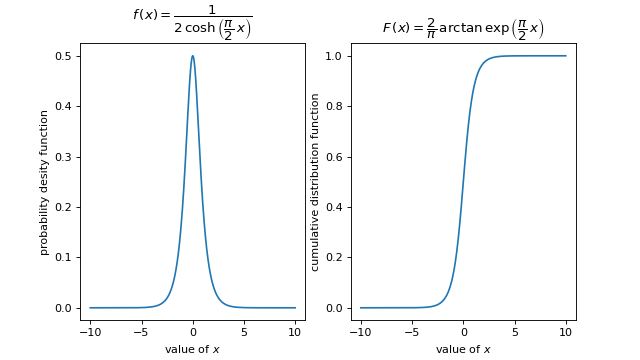
\includegraphics[scale=0.595]{fig1.png}
	Example: Let $u = 0.8$ , From above equations: $x_{0.8} = 0.716, x_{0.2} = -0.716 $\\
	Hence Verified.
\end{frame}

\end{document}